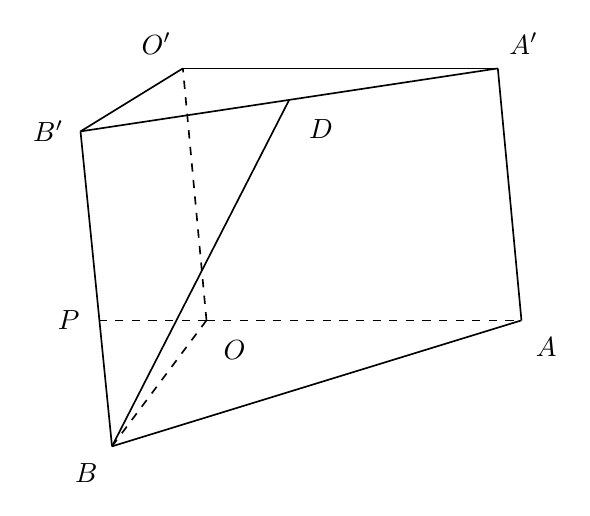
\begin{tikzpicture}[x=1cm,y=1cm,font=\normalsize]
\tikzset{solid edge/.style={draw=black,solid,line width=.6pt},dashed edge/.style={draw=black,dashed,line width=.6pt},pt label/.style={font=\normalsize,inner sep=2pt}}
\coordinate (O) at (0,0);
\coordinate (A) at (4,0);
\coordinate (B) at (-1.2,-1.6);
\coordinate (Oprime) at (-0.3,3.2);
\coordinate (Aprime) at (3.7,3.2);
\coordinate (Bprime) at (-1.6,2.4);
\coordinate (P) at (-1.36,0);
\coordinate (D) at (1.05,2.8);
\draw[dashed edge] (O) -- (A);
\draw[dashed edge] (O) -- (B);
\draw[dashed edge] (O) -- (Oprime);
\draw[dashed edge] (O) -- (P);
\draw[solid edge] (A) -- (B);
\draw[solid edge] (A) -- (Aprime);
\draw[solid edge] (B) -- (Bprime);
\draw[solid edge] (B) -- (D);
\draw[solid edge] (Oprime) -- (Aprime);
\draw[solid edge] (Oprime) -- (Bprime);
\draw[solid edge] (Bprime) -- (Aprime);
\node[pt label,above left,xshift=-2pt,yshift=3pt] at (Oprime) {$O'$};
\node[pt label,above right,xshift=2pt,yshift=3pt] at (Aprime) {$A'$};
\node[pt label,left,xshift=-4pt] at (Bprime) {$B'$};
\node[pt label,below right,xshift=5pt,yshift=-5pt] at (D) {$D$};
\node[pt label,left,xshift=-5pt] at (P) {$P$};
\node[pt label,below right,xshift=4pt,yshift=-5pt] at (O) {$O$};
\node[pt label,below right,xshift=3pt,yshift=-4pt] at (A) {$A$};
\node[pt label,below left,xshift=-3pt,yshift=-4pt] at (B) {$B$};
\end{tikzpicture}
